% Options for packages loaded elsewhere
\PassOptionsToPackage{unicode}{hyperref}
\PassOptionsToPackage{hyphens}{url}
%
\documentclass[
]{article}
\usepackage{amsmath,amssymb}
\usepackage{lmodern}
\usepackage{iftex}
\ifPDFTeX
  \usepackage[T1]{fontenc}
  \usepackage[utf8]{inputenc}
  \usepackage{textcomp} % provide euro and other symbols
\else % if luatex or xetex
  \usepackage{unicode-math}
  \defaultfontfeatures{Scale=MatchLowercase}
  \defaultfontfeatures[\rmfamily]{Ligatures=TeX,Scale=1}
\fi
% Use upquote if available, for straight quotes in verbatim environments
\IfFileExists{upquote.sty}{\usepackage{upquote}}{}
\IfFileExists{microtype.sty}{% use microtype if available
  \usepackage[]{microtype}
  \UseMicrotypeSet[protrusion]{basicmath} % disable protrusion for tt fonts
}{}
\makeatletter
\@ifundefined{KOMAClassName}{% if non-KOMA class
  \IfFileExists{parskip.sty}{%
    \usepackage{parskip}
  }{% else
    \setlength{\parindent}{0pt}
    \setlength{\parskip}{6pt plus 2pt minus 1pt}}
}{% if KOMA class
  \KOMAoptions{parskip=half}}
\makeatother
\usepackage{xcolor}
\usepackage[margin=1in]{geometry}
\usepackage{color}
\usepackage{fancyvrb}
\newcommand{\VerbBar}{|}
\newcommand{\VERB}{\Verb[commandchars=\\\{\}]}
\DefineVerbatimEnvironment{Highlighting}{Verbatim}{commandchars=\\\{\}}
% Add ',fontsize=\small' for more characters per line
\usepackage{framed}
\definecolor{shadecolor}{RGB}{248,248,248}
\newenvironment{Shaded}{\begin{snugshade}}{\end{snugshade}}
\newcommand{\AlertTok}[1]{\textcolor[rgb]{0.94,0.16,0.16}{#1}}
\newcommand{\AnnotationTok}[1]{\textcolor[rgb]{0.56,0.35,0.01}{\textbf{\textit{#1}}}}
\newcommand{\AttributeTok}[1]{\textcolor[rgb]{0.77,0.63,0.00}{#1}}
\newcommand{\BaseNTok}[1]{\textcolor[rgb]{0.00,0.00,0.81}{#1}}
\newcommand{\BuiltInTok}[1]{#1}
\newcommand{\CharTok}[1]{\textcolor[rgb]{0.31,0.60,0.02}{#1}}
\newcommand{\CommentTok}[1]{\textcolor[rgb]{0.56,0.35,0.01}{\textit{#1}}}
\newcommand{\CommentVarTok}[1]{\textcolor[rgb]{0.56,0.35,0.01}{\textbf{\textit{#1}}}}
\newcommand{\ConstantTok}[1]{\textcolor[rgb]{0.00,0.00,0.00}{#1}}
\newcommand{\ControlFlowTok}[1]{\textcolor[rgb]{0.13,0.29,0.53}{\textbf{#1}}}
\newcommand{\DataTypeTok}[1]{\textcolor[rgb]{0.13,0.29,0.53}{#1}}
\newcommand{\DecValTok}[1]{\textcolor[rgb]{0.00,0.00,0.81}{#1}}
\newcommand{\DocumentationTok}[1]{\textcolor[rgb]{0.56,0.35,0.01}{\textbf{\textit{#1}}}}
\newcommand{\ErrorTok}[1]{\textcolor[rgb]{0.64,0.00,0.00}{\textbf{#1}}}
\newcommand{\ExtensionTok}[1]{#1}
\newcommand{\FloatTok}[1]{\textcolor[rgb]{0.00,0.00,0.81}{#1}}
\newcommand{\FunctionTok}[1]{\textcolor[rgb]{0.00,0.00,0.00}{#1}}
\newcommand{\ImportTok}[1]{#1}
\newcommand{\InformationTok}[1]{\textcolor[rgb]{0.56,0.35,0.01}{\textbf{\textit{#1}}}}
\newcommand{\KeywordTok}[1]{\textcolor[rgb]{0.13,0.29,0.53}{\textbf{#1}}}
\newcommand{\NormalTok}[1]{#1}
\newcommand{\OperatorTok}[1]{\textcolor[rgb]{0.81,0.36,0.00}{\textbf{#1}}}
\newcommand{\OtherTok}[1]{\textcolor[rgb]{0.56,0.35,0.01}{#1}}
\newcommand{\PreprocessorTok}[1]{\textcolor[rgb]{0.56,0.35,0.01}{\textit{#1}}}
\newcommand{\RegionMarkerTok}[1]{#1}
\newcommand{\SpecialCharTok}[1]{\textcolor[rgb]{0.00,0.00,0.00}{#1}}
\newcommand{\SpecialStringTok}[1]{\textcolor[rgb]{0.31,0.60,0.02}{#1}}
\newcommand{\StringTok}[1]{\textcolor[rgb]{0.31,0.60,0.02}{#1}}
\newcommand{\VariableTok}[1]{\textcolor[rgb]{0.00,0.00,0.00}{#1}}
\newcommand{\VerbatimStringTok}[1]{\textcolor[rgb]{0.31,0.60,0.02}{#1}}
\newcommand{\WarningTok}[1]{\textcolor[rgb]{0.56,0.35,0.01}{\textbf{\textit{#1}}}}
\usepackage{graphicx}
\makeatletter
\def\maxwidth{\ifdim\Gin@nat@width>\linewidth\linewidth\else\Gin@nat@width\fi}
\def\maxheight{\ifdim\Gin@nat@height>\textheight\textheight\else\Gin@nat@height\fi}
\makeatother
% Scale images if necessary, so that they will not overflow the page
% margins by default, and it is still possible to overwrite the defaults
% using explicit options in \includegraphics[width, height, ...]{}
\setkeys{Gin}{width=\maxwidth,height=\maxheight,keepaspectratio}
% Set default figure placement to htbp
\makeatletter
\def\fps@figure{htbp}
\makeatother
\setlength{\emergencystretch}{3em} % prevent overfull lines
\providecommand{\tightlist}{%
  \setlength{\itemsep}{0pt}\setlength{\parskip}{0pt}}
\setcounter{secnumdepth}{-\maxdimen} % remove section numbering
\ifLuaTeX
  \usepackage{selnolig}  % disable illegal ligatures
\fi
\IfFileExists{bookmark.sty}{\usepackage{bookmark}}{\usepackage{hyperref}}
\IfFileExists{xurl.sty}{\usepackage{xurl}}{} % add URL line breaks if available
\urlstyle{same} % disable monospaced font for URLs
\hypersetup{
  pdftitle={Paper 2, Econ 980x},
  pdfauthor={Alice Chen},
  hidelinks,
  pdfcreator={LaTeX via pandoc}}

\title{Paper 2, Econ 980x}
\author{Alice Chen}
\date{2022-11-27}

\begin{document}
\maketitle

\begin{Shaded}
\begin{Highlighting}[]
\NormalTok{csv }\OtherTok{\textless{}{-}} \FunctionTok{read\_csv}\NormalTok{(}\AttributeTok{file =} \StringTok{"atus\_00001.csv.gz"}\NormalTok{) }\SpecialCharTok{\%\textgreater{}\%}
  \FunctionTok{clean\_names}\NormalTok{()}
\end{Highlighting}
\end{Shaded}

\begin{verbatim}
## Rows: 228455 Columns: 38
## -- Column specification --------------------------------------------------------
## Delimiter: ","
## dbl (38): YEAR, CASEID, PERNUM, LINENO, WT06, WT20, AGE, SEX, RACE, MARST, E...
## 
## i Use `spec()` to retrieve the full column specification for this data.
## i Specify the column types or set `show_col_types = FALSE` to quiet this message.
\end{verbatim}

\begin{Shaded}
\begin{Highlighting}[]
\CommentTok{\# race }
\NormalTok{race\_file }\OtherTok{\textless{}{-}} \FunctionTok{read\_excel}\NormalTok{(}\StringTok{"race\_980x.xlsx"}\NormalTok{)}

\NormalTok{race\_file }\OtherTok{\textless{}{-}}\NormalTok{ race\_file }\SpecialCharTok{\%\textgreater{}\%}
  \FunctionTok{rename}\NormalTok{(}\AttributeTok{code1 =}\NormalTok{ race) }\SpecialCharTok{\%\textgreater{}\%}
  \FunctionTok{rename}\NormalTok{(}\AttributeTok{race =}\NormalTok{ code) }

\NormalTok{csv }\OtherTok{\textless{}{-}} \FunctionTok{left\_join}\NormalTok{(csv, race\_file, }\AttributeTok{by =} \StringTok{"race"}\NormalTok{) }\SpecialCharTok{\%\textgreater{}\%}
  \FunctionTok{rename}\NormalTok{(}\AttributeTok{race\_code =}\NormalTok{ race) }\SpecialCharTok{\%\textgreater{}\%}
  \FunctionTok{rename}\NormalTok{(}\AttributeTok{race =}\NormalTok{ code1)}


\CommentTok{\# education}
\NormalTok{education\_file }\OtherTok{\textless{}{-}} \FunctionTok{read\_excel}\NormalTok{(}\StringTok{"Education.xlsx"}\NormalTok{)}
\NormalTok{education\_file }\OtherTok{\textless{}{-}}\NormalTok{ education\_file }\SpecialCharTok{\%\textgreater{}\%}
  \FunctionTok{rename}\NormalTok{(}\AttributeTok{code\_educ =}\NormalTok{ educ) }\SpecialCharTok{\%\textgreater{}\%}
  \FunctionTok{rename}\NormalTok{(}\AttributeTok{educ =}\NormalTok{ code\_education) }\SpecialCharTok{\%\textgreater{}\%}
  \FunctionTok{mutate}\NormalTok{(}\AttributeTok{educ =} \FunctionTok{as.numeric}\NormalTok{(educ))}

\NormalTok{csv }\OtherTok{\textless{}{-}} \FunctionTok{left\_join}\NormalTok{(csv, education\_file, }\AttributeTok{by =} \StringTok{"educ"}\NormalTok{) }\SpecialCharTok{\%\textgreater{}\%}
  \FunctionTok{rename}\NormalTok{(}\AttributeTok{code\_education =}\NormalTok{ educ) }\SpecialCharTok{\%\textgreater{}\%}
  \FunctionTok{rename}\NormalTok{(}\AttributeTok{educ =}\NormalTok{ code\_educ) }

\CommentTok{\# marital status}
\NormalTok{marital\_file }\OtherTok{\textless{}{-}} \FunctionTok{read\_excel}\NormalTok{(}\StringTok{"marital\_status.xlsx"}\NormalTok{)}
\NormalTok{education\_file }\OtherTok{\textless{}{-}}\NormalTok{ marital\_file }\SpecialCharTok{\%\textgreater{}\%}
  \FunctionTok{mutate}\NormalTok{(}\AttributeTok{marst =} \FunctionTok{as.numeric}\NormalTok{(marst))}
  
\NormalTok{csv }\OtherTok{\textless{}{-}} \FunctionTok{left\_join}\NormalTok{(csv, marital\_file, }\AttributeTok{by =} \StringTok{"marst"}\NormalTok{) }\SpecialCharTok{\%\textgreater{}\%}
  \FunctionTok{rename}\NormalTok{(}\AttributeTok{code\_marst =}\NormalTok{ marst) }\SpecialCharTok{\%\textgreater{}\%}
  \FunctionTok{rename}\NormalTok{(}\AttributeTok{marst =}\NormalTok{ marst\_code) }\SpecialCharTok{\%\textgreater{}\%}
  \FunctionTok{mutate}\NormalTok{(}\AttributeTok{marst\_simple =} \FunctionTok{ifelse}\NormalTok{(code\_marst }\SpecialCharTok{\textless{}=} \DecValTok{2}\NormalTok{, }\StringTok{"Married"}\NormalTok{, }\FunctionTok{ifelse}\NormalTok{(code\_marst }\SpecialCharTok{\textgreater{}=} \DecValTok{6}\NormalTok{, }\StringTok{"Never Married"}\NormalTok{, }\StringTok{"Separated/Divorced"}\NormalTok{)))}



\CommentTok{\# age}
\NormalTok{csv }\OtherTok{\textless{}{-}}\NormalTok{ csv }\SpecialCharTok{\%\textgreater{}\%}
  \FunctionTok{filter}\NormalTok{(age }\SpecialCharTok{\textgreater{}} \DecValTok{18}\NormalTok{)}

\CommentTok{\# children}
\NormalTok{csv }\OtherTok{\textless{}{-}}\NormalTok{ csv }\SpecialCharTok{\%\textgreater{}\%}
  \FunctionTok{mutate}\NormalTok{(}\AttributeTok{child =} \FunctionTok{ifelse}\NormalTok{(yngch }\SpecialCharTok{\textless{}} \DecValTok{19}\NormalTok{, }\DecValTok{1}\NormalTok{, }\DecValTok{0}\NormalTok{) )}

\CommentTok{\# gender}

\NormalTok{csv }\OtherTok{\textless{}{-}}\NormalTok{ csv }\SpecialCharTok{\%\textgreater{}\%}
  \FunctionTok{mutate}\NormalTok{(}\AttributeTok{gender =} \FunctionTok{ifelse}\NormalTok{(sex }\SpecialCharTok{==} \DecValTok{1}\NormalTok{, }\StringTok{"male"}\NormalTok{, }\StringTok{"female"}\NormalTok{)) }

\CommentTok{\# years }
\end{Highlighting}
\end{Shaded}

\begin{Shaded}
\begin{Highlighting}[]
\CommentTok{\#leisure hours aggregate}
\NormalTok{csv }\SpecialCharTok{\%\textgreater{}\%}
  \FunctionTok{ggplot}\NormalTok{(}\AttributeTok{mapping =} \FunctionTok{aes}\NormalTok{(}\AttributeTok{x =}\NormalTok{ bls\_leis)) }\SpecialCharTok{+}
  \FunctionTok{geom\_histogram}\NormalTok{(}\AttributeTok{binwidth=}\DecValTok{50}\NormalTok{) }\SpecialCharTok{+}
  \FunctionTok{labs}\NormalTok{(}
  \AttributeTok{title =} \StringTok{"Distribution of annual individual leisure hours"}\NormalTok{,}
  \AttributeTok{x =} \StringTok{"Annual Hours"}\NormalTok{,}
  \AttributeTok{y =} \StringTok{"Count"}\NormalTok{,}
  \AttributeTok{caption =} \StringTok{"Data from ATUS"}\NormalTok{,}
\NormalTok{) }
\end{Highlighting}
\end{Shaded}

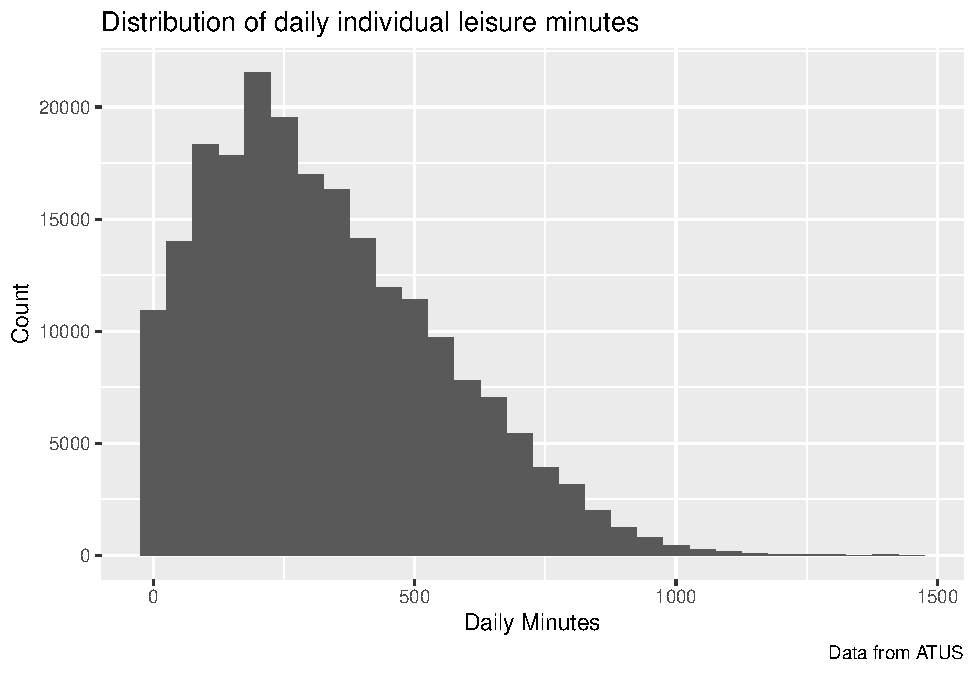
\includegraphics{Paper2_files/figure-latex/graphs-1.pdf}

\begin{Shaded}
\begin{Highlighting}[]
\NormalTok{csv }\SpecialCharTok{\%\textgreater{}\%}
  \FunctionTok{filter}\NormalTok{(year }\SpecialCharTok{\%in\%} \FunctionTok{c}\NormalTok{(}\DecValTok{2007}\NormalTok{, }\DecValTok{2009}\NormalTok{)) }\SpecialCharTok{\%\textgreater{}\%}
  \FunctionTok{ggplot}\NormalTok{(}\AttributeTok{mapping =} \FunctionTok{aes}\NormalTok{(}\AttributeTok{x =}\NormalTok{ bls\_leis)) }\SpecialCharTok{+}
  \FunctionTok{geom\_histogram}\NormalTok{(}\AttributeTok{binwidth=}\DecValTok{50}\NormalTok{) }\SpecialCharTok{+}
  \FunctionTok{facet\_wrap}\NormalTok{(}\SpecialCharTok{\textasciitilde{}}\NormalTok{year) }\SpecialCharTok{+}
  \FunctionTok{labs}\NormalTok{(}
  \AttributeTok{title =} \StringTok{"Distribution of annual individual leisure hours"}\NormalTok{,}
  \AttributeTok{x =} \StringTok{"Annual Hours"}\NormalTok{,}
  \AttributeTok{y =} \StringTok{"Count"}\NormalTok{,}
  \AttributeTok{caption =} \StringTok{"Data from ATUS"}\NormalTok{,}
\NormalTok{)}
\end{Highlighting}
\end{Shaded}

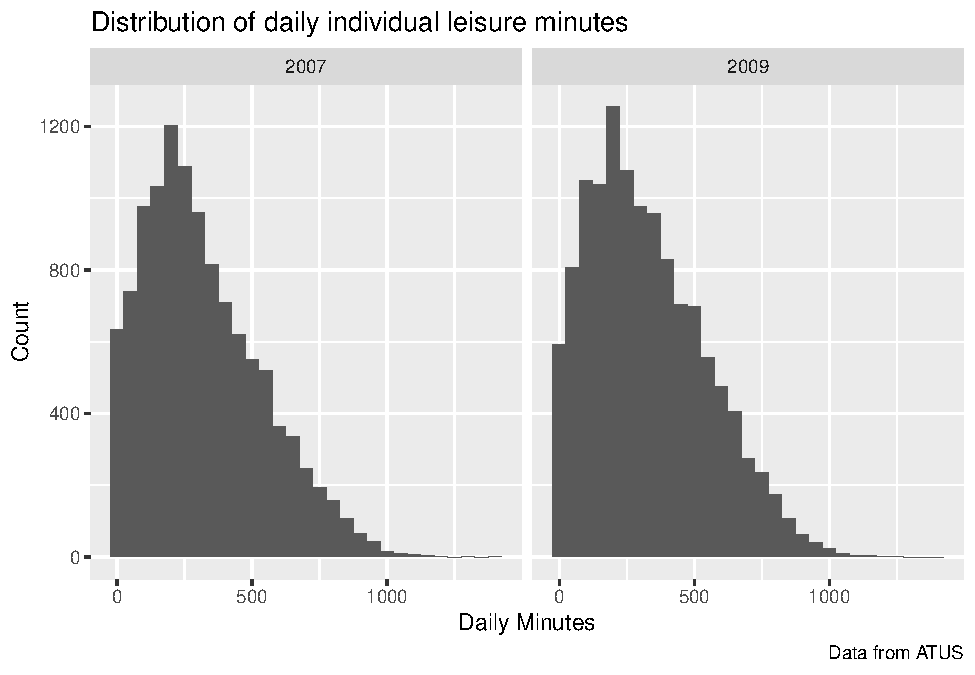
\includegraphics{Paper2_files/figure-latex/graphs-2.pdf}

\begin{Shaded}
\begin{Highlighting}[]
\CommentTok{\#leisure hours aggregate by gender}
\NormalTok{csv }\SpecialCharTok{\%\textgreater{}\%}
  \FunctionTok{group\_by}\NormalTok{(gender) }\SpecialCharTok{\%\textgreater{}\%}
  \FunctionTok{ggplot}\NormalTok{(}\AttributeTok{mapping =} \FunctionTok{aes}\NormalTok{(}\AttributeTok{x =}\NormalTok{ bls\_leis) )}\SpecialCharTok{+}
  \FunctionTok{geom\_histogram}\NormalTok{(}\AttributeTok{binwidth=}\DecValTok{50}\NormalTok{) }\SpecialCharTok{+}
  \FunctionTok{facet\_wrap}\NormalTok{(}\SpecialCharTok{\textasciitilde{}}\NormalTok{ gender) }\SpecialCharTok{+}
    \FunctionTok{labs}\NormalTok{(}
  \AttributeTok{title =} \StringTok{"Distribution of annual individual leisure hours by gender"}\NormalTok{,}
  \AttributeTok{x =} \StringTok{"Annual Hours"}\NormalTok{,}
  \AttributeTok{y =} \StringTok{"Count"}\NormalTok{,}
  \AttributeTok{caption =} \StringTok{"Data from ATUS"}\NormalTok{,}
\NormalTok{)}
\end{Highlighting}
\end{Shaded}

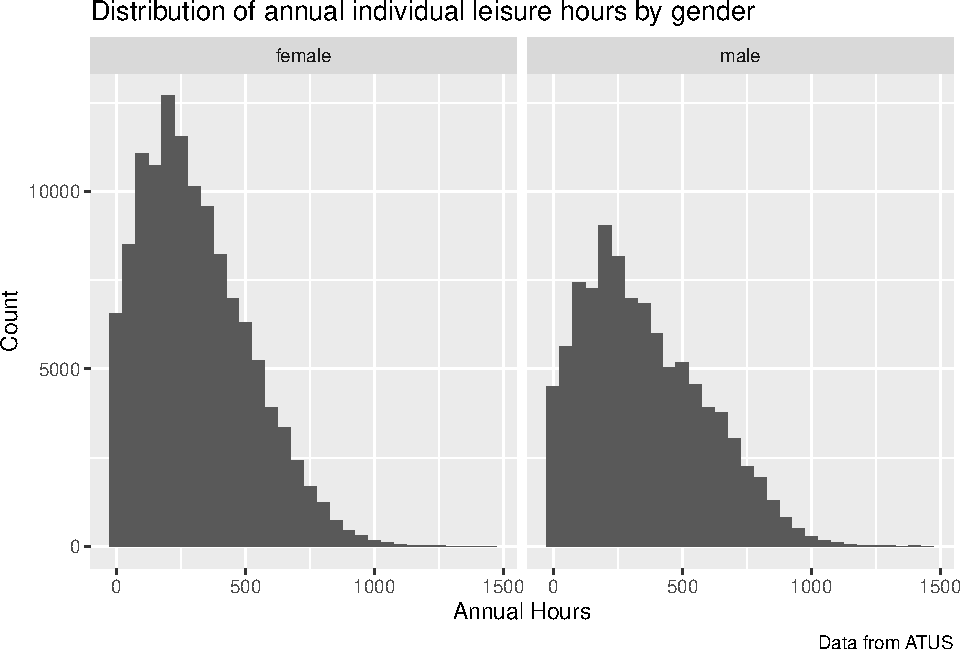
\includegraphics{Paper2_files/figure-latex/graphs-3.pdf}

\begin{Shaded}
\begin{Highlighting}[]
\NormalTok{csv }\SpecialCharTok{\%\textgreater{}\%}
  \FunctionTok{filter}\NormalTok{(year }\SpecialCharTok{\%in\%} \FunctionTok{c}\NormalTok{(}\DecValTok{2007}\NormalTok{, }\DecValTok{2009}\NormalTok{)) }\SpecialCharTok{\%\textgreater{}\%}
  \FunctionTok{ggplot}\NormalTok{(}\AttributeTok{mapping =} \FunctionTok{aes}\NormalTok{(}\AttributeTok{x =}\NormalTok{ bls\_leis)) }\SpecialCharTok{+}
  \FunctionTok{geom\_histogram}\NormalTok{(}\AttributeTok{binwidth=}\DecValTok{50}\NormalTok{) }\SpecialCharTok{+}
  \FunctionTok{facet\_wrap}\NormalTok{(}\SpecialCharTok{\textasciitilde{}}\NormalTok{ gender }\SpecialCharTok{+}\NormalTok{ year) }\SpecialCharTok{+}
  \FunctionTok{labs}\NormalTok{(}
  \AttributeTok{title =} \StringTok{"Distribution of annual individual leisure hours by gender"}\NormalTok{,}
  \AttributeTok{x =} \StringTok{"Annual Hours"}\NormalTok{,}
  \AttributeTok{y =} \StringTok{"Count"}\NormalTok{,}
  \AttributeTok{caption =} \StringTok{"Data from ATUS"}\NormalTok{,}
\NormalTok{)}
\end{Highlighting}
\end{Shaded}

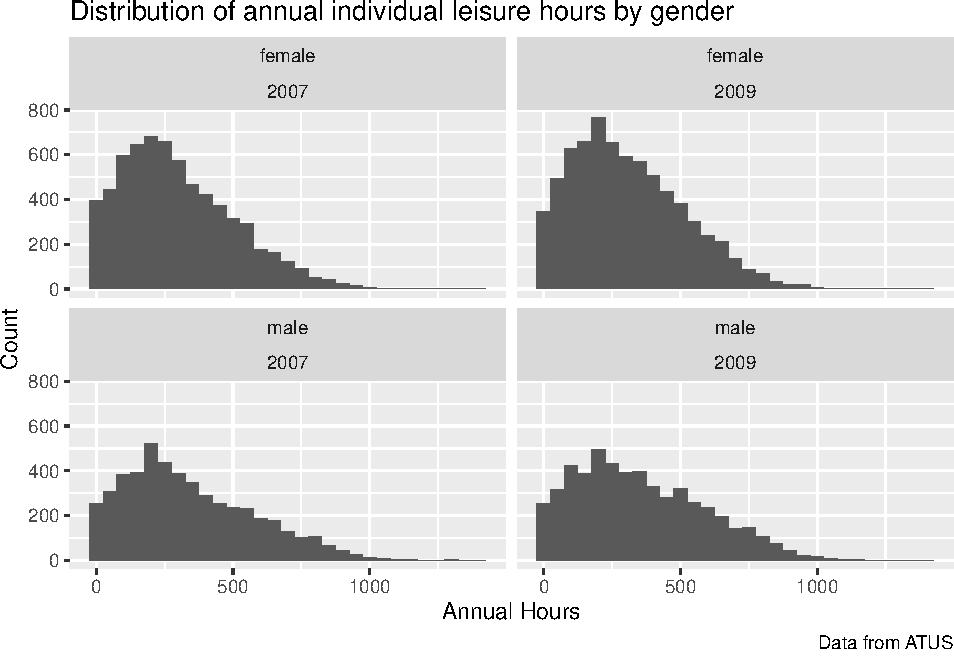
\includegraphics{Paper2_files/figure-latex/graphs-4.pdf}

\begin{Shaded}
\begin{Highlighting}[]
\CommentTok{\# Median}
\NormalTok{csv }\SpecialCharTok{\%\textgreater{}\%}
  \FunctionTok{group\_by}\NormalTok{(year, gender) }\SpecialCharTok{\%\textgreater{}\%}
  \FunctionTok{summarize}\NormalTok{(}\FunctionTok{median}\NormalTok{(bls\_leis)) }\SpecialCharTok{\%\textgreater{}\%}
  \FunctionTok{clean\_names}\NormalTok{() }\SpecialCharTok{\%\textgreater{}\%}
  \FunctionTok{ggplot}\NormalTok{(}\FunctionTok{aes}\NormalTok{(}\AttributeTok{x =}\NormalTok{ year, }\AttributeTok{y =}\NormalTok{ median\_bls\_leis)) }\SpecialCharTok{+}
  \FunctionTok{geom\_line}\NormalTok{() }\SpecialCharTok{+}
  \FunctionTok{facet\_wrap}\NormalTok{(}\SpecialCharTok{\textasciitilde{}}\NormalTok{ gender) }\SpecialCharTok{+}
  \FunctionTok{labs}\NormalTok{(}
  \AttributeTok{title =} \StringTok{"Median annual individual leisure hours by gender"}\NormalTok{,}
  \AttributeTok{y =} \StringTok{"Annual Hours"}\NormalTok{,}
  \AttributeTok{x =} \StringTok{"Year"}\NormalTok{,}
  \AttributeTok{caption =} \StringTok{"Data from ATUS"}\NormalTok{,}
\NormalTok{) }
\end{Highlighting}
\end{Shaded}

\begin{verbatim}
## `summarise()` has grouped output by 'year'. You can override using the
## `.groups` argument.
\end{verbatim}

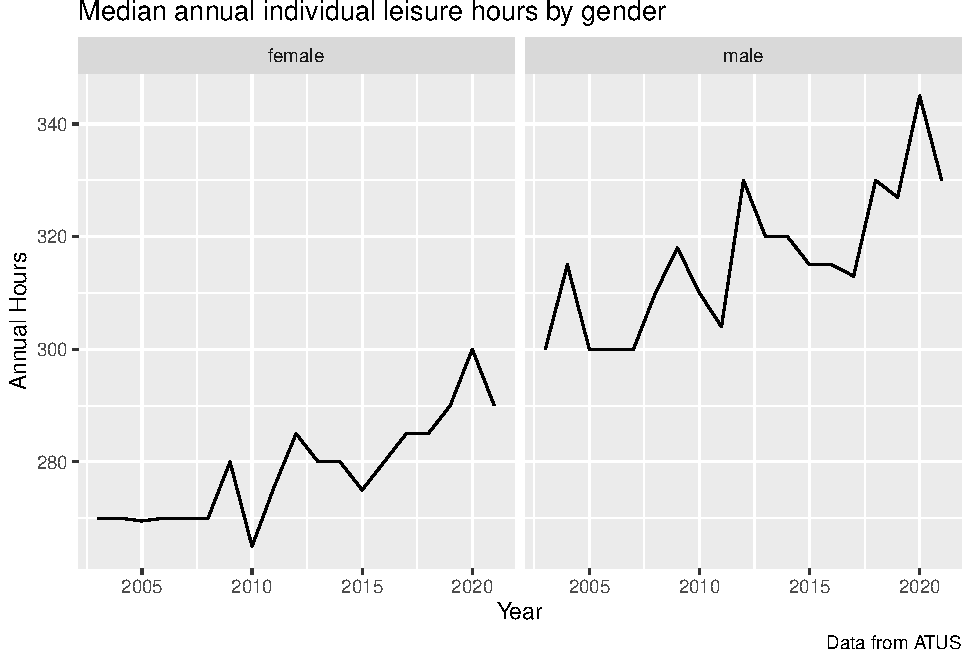
\includegraphics{Paper2_files/figure-latex/graphs-5.pdf}

\begin{Shaded}
\begin{Highlighting}[]
\CommentTok{\# All Quantile}
\NormalTok{csv }\SpecialCharTok{\%\textgreater{}\%}
  \FunctionTok{group\_by}\NormalTok{(year, gender) }\SpecialCharTok{\%\textgreater{}\%}
  \FunctionTok{summarize}\NormalTok{(}\AttributeTok{quantile\_25 =} \FunctionTok{quantile}\NormalTok{(bls\_leis, }\FloatTok{0.25}\NormalTok{), }\AttributeTok{quantile\_50 =} \FunctionTok{quantile}\NormalTok{(bls\_leis, }\FloatTok{0.5}\NormalTok{), }\AttributeTok{quantile\_75 =} \FunctionTok{quantile}\NormalTok{(bls\_leis, }\FloatTok{0.75}\NormalTok{)) }\SpecialCharTok{\%\textgreater{}\%}
  \FunctionTok{clean\_names}\NormalTok{() }\SpecialCharTok{\%\textgreater{}\%}
  \FunctionTok{pivot\_longer}\NormalTok{(quantile\_25}\SpecialCharTok{:}\NormalTok{quantile\_75, }\AttributeTok{names\_to =} \StringTok{"quantile"}\NormalTok{, }\AttributeTok{values\_to =} \StringTok{"hours"}\NormalTok{) }\SpecialCharTok{\%\textgreater{}\%}
  \FunctionTok{ggplot}\NormalTok{(}\FunctionTok{aes}\NormalTok{(}\AttributeTok{x =}\NormalTok{ year, }\AttributeTok{y =}\NormalTok{ hours, }\AttributeTok{group =}\NormalTok{ quantile, }\AttributeTok{colour =}\NormalTok{ quantile)) }\SpecialCharTok{+}
  \FunctionTok{geom\_line}\NormalTok{() }\SpecialCharTok{+}
    \FunctionTok{facet\_wrap}\NormalTok{(}\SpecialCharTok{\textasciitilde{}}\NormalTok{ gender) }\SpecialCharTok{+}
  \FunctionTok{labs}\NormalTok{(}
  \AttributeTok{title =} \StringTok{"Annual individual leisure hours by gender"}\NormalTok{,}
  \AttributeTok{y =} \StringTok{"Annual Hours"}\NormalTok{,}
  \AttributeTok{x =} \StringTok{"Year"}\NormalTok{,}
  \AttributeTok{caption =} \StringTok{"Data from ATUS"}\NormalTok{,}
\NormalTok{) }
\end{Highlighting}
\end{Shaded}

\begin{verbatim}
## `summarise()` has grouped output by 'year'. You can override using the
## `.groups` argument.
\end{verbatim}

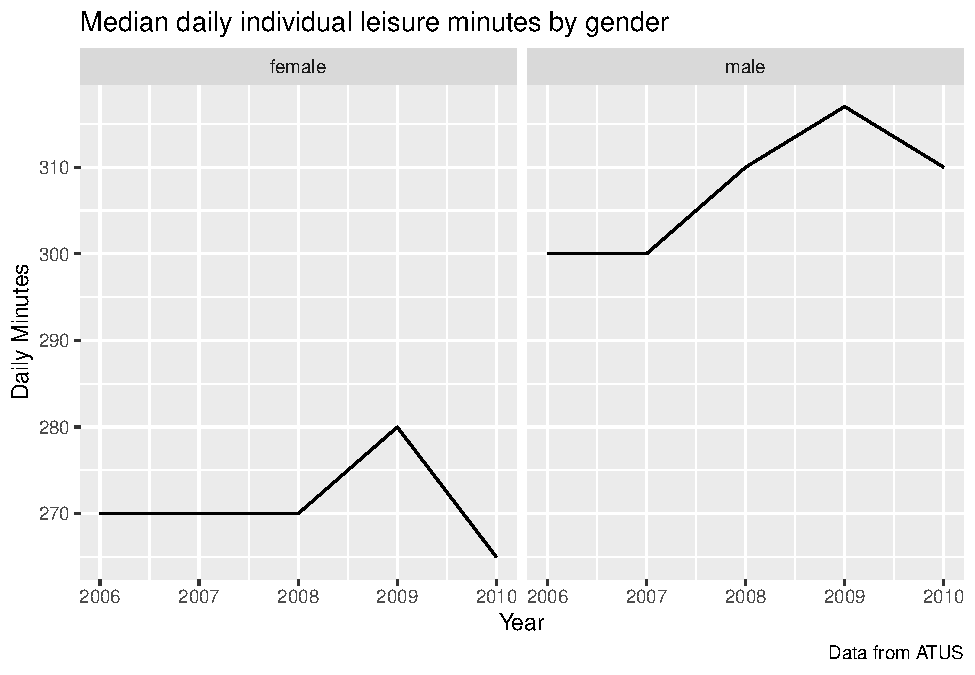
\includegraphics{Paper2_files/figure-latex/graphs-6.pdf}

\begin{Shaded}
\begin{Highlighting}[]
\NormalTok{csv }\SpecialCharTok{\%\textgreater{}\%}
  \FunctionTok{group\_by}\NormalTok{(year) }\SpecialCharTok{\%\textgreater{}\%}
  \FunctionTok{summarize}\NormalTok{(}\FunctionTok{quantile}\NormalTok{(bls\_leis, }\FloatTok{0.25}\NormalTok{), }\FunctionTok{quantile}\NormalTok{(bls\_leis, }\FloatTok{0.5}\NormalTok{), }\FunctionTok{quantile}\NormalTok{(bls\_leis, }\FloatTok{0.75}\NormalTok{)) }\SpecialCharTok{\%\textgreater{}\%}
  \FunctionTok{clean\_names}\NormalTok{() }\SpecialCharTok{\%\textgreater{}\%}
  \FunctionTok{pivot\_longer}\NormalTok{(}\SpecialCharTok{!}\NormalTok{year, }\AttributeTok{names\_to =} \StringTok{"quantile"}\NormalTok{, }\AttributeTok{values\_to =} \StringTok{"hours"}\NormalTok{) }\SpecialCharTok{\%\textgreater{}\%}
  \FunctionTok{ggplot}\NormalTok{(}\FunctionTok{aes}\NormalTok{(}\AttributeTok{x =}\NormalTok{ year, }\AttributeTok{y =}\NormalTok{ hours, }\AttributeTok{group =}\NormalTok{ quantile)) }\SpecialCharTok{+}
  \FunctionTok{geom\_line}\NormalTok{()}
\end{Highlighting}
\end{Shaded}

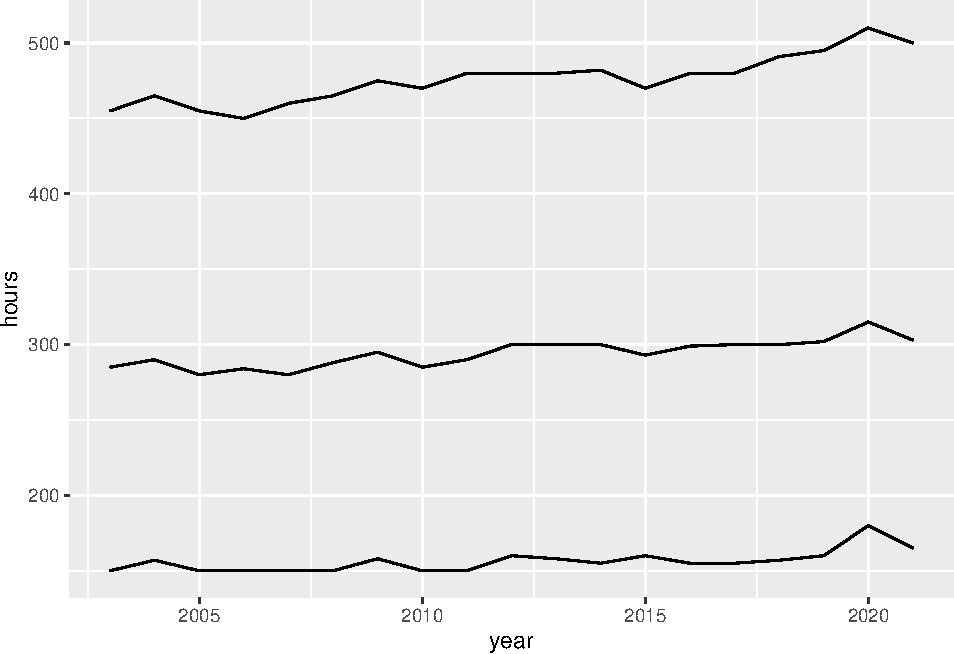
\includegraphics{Paper2_files/figure-latex/graphs-7.pdf}

\begin{Shaded}
\begin{Highlighting}[]
\NormalTok{csv }\SpecialCharTok{\%\textgreater{}\%}
  \FunctionTok{group\_by}\NormalTok{(year) }\SpecialCharTok{\%\textgreater{}\%}
  \FunctionTok{summarize}\NormalTok{(}\FunctionTok{quantile}\NormalTok{(bls\_leis, }\FloatTok{0.25}\NormalTok{), }\FunctionTok{quantile}\NormalTok{(bls\_leis, }\FloatTok{0.5}\NormalTok{), }\FunctionTok{quantile}\NormalTok{(bls\_leis, }\FloatTok{0.75}\NormalTok{)) }\SpecialCharTok{\%\textgreater{}\%}
  \FunctionTok{clean\_names}\NormalTok{() }\SpecialCharTok{\%\textgreater{}\%}
  \FunctionTok{pivot\_longer}\NormalTok{(}\SpecialCharTok{!}\NormalTok{year, }\AttributeTok{names\_to =} \StringTok{"quantile"}\NormalTok{, }\AttributeTok{values\_to =} \StringTok{"hours"}\NormalTok{) }\SpecialCharTok{\%\textgreater{}\%}
  \FunctionTok{filter}\NormalTok{(year }\SpecialCharTok{\textgreater{}} \DecValTok{2006}\NormalTok{) }\SpecialCharTok{\%\textgreater{}\%}
  \FunctionTok{filter}\NormalTok{(year }\SpecialCharTok{\textless{}} \DecValTok{2011}\NormalTok{) }\SpecialCharTok{\%\textgreater{}\%}
  \FunctionTok{ggplot}\NormalTok{(}\FunctionTok{aes}\NormalTok{(}\AttributeTok{x =}\NormalTok{ year, }\AttributeTok{y =}\NormalTok{ hours, }\AttributeTok{group =}\NormalTok{ quantile)) }\SpecialCharTok{+}
  \FunctionTok{geom\_line}\NormalTok{()}
\end{Highlighting}
\end{Shaded}

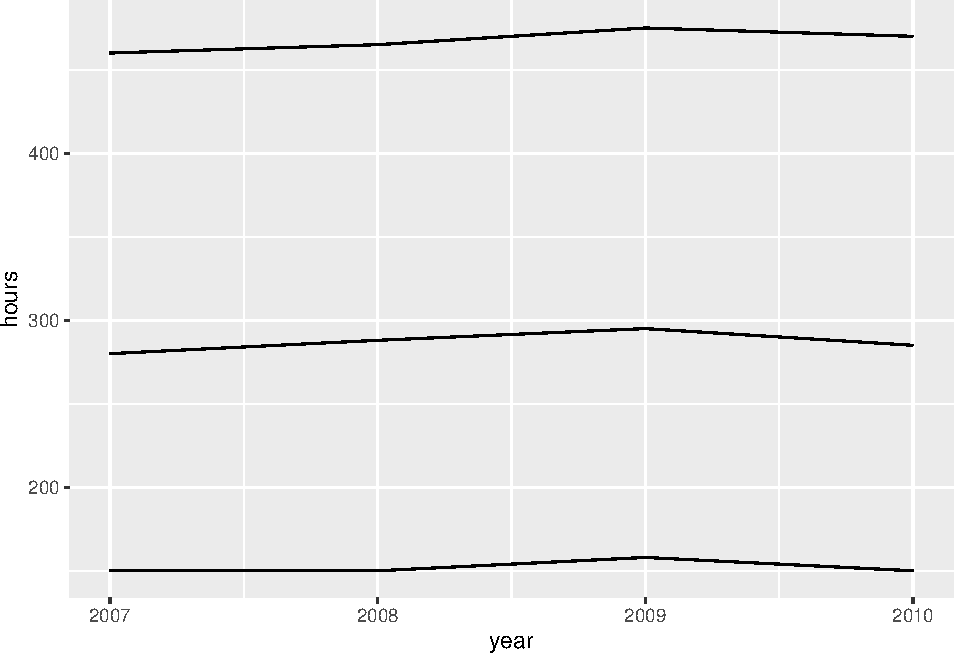
\includegraphics{Paper2_files/figure-latex/graphs-8.pdf}

\begin{Shaded}
\begin{Highlighting}[]
\CommentTok{\# by year, gender}
\NormalTok{csv }\SpecialCharTok{\%\textgreater{}\%}
  \FunctionTok{group\_by}\NormalTok{(year, gender) }\SpecialCharTok{\%\textgreater{}\%}
  \FunctionTok{summarize}\NormalTok{(}\AttributeTok{quantile\_25 =} \FunctionTok{quantile}\NormalTok{(bls\_leis, }\FloatTok{0.25}\NormalTok{), }\AttributeTok{quantile\_50 =} \FunctionTok{quantile}\NormalTok{(bls\_leis, }\FloatTok{0.5}\NormalTok{), }\AttributeTok{quantile\_75 =} \FunctionTok{quantile}\NormalTok{(bls\_leis, }\FloatTok{0.75}\NormalTok{)) }\SpecialCharTok{\%\textgreater{}\%}
  \FunctionTok{clean\_names}\NormalTok{() }\SpecialCharTok{\%\textgreater{}\%}
  \FunctionTok{pivot\_longer}\NormalTok{(quantile\_25}\SpecialCharTok{:}\NormalTok{quantile\_75, }\AttributeTok{names\_to =} \StringTok{"quantile"}\NormalTok{, }\AttributeTok{values\_to =} \StringTok{"hours"}\NormalTok{) }\SpecialCharTok{\%\textgreater{}\%}
  \FunctionTok{filter}\NormalTok{(year }\SpecialCharTok{\textgreater{}} \DecValTok{2005}\NormalTok{) }\SpecialCharTok{\%\textgreater{}\%}
  \FunctionTok{filter}\NormalTok{(year }\SpecialCharTok{\textless{}} \DecValTok{2011}\NormalTok{) }\SpecialCharTok{\%\textgreater{}\%}
  \FunctionTok{ggplot}\NormalTok{(}\FunctionTok{aes}\NormalTok{(}\AttributeTok{x =}\NormalTok{ year, }\AttributeTok{y =}\NormalTok{ hours, }\AttributeTok{group =}\NormalTok{ quantile, }\AttributeTok{colour =}\NormalTok{ quantile)) }\SpecialCharTok{+}
  \FunctionTok{geom\_line}\NormalTok{() }\SpecialCharTok{+}
  \FunctionTok{facet\_wrap}\NormalTok{(}\SpecialCharTok{\textasciitilde{}}\NormalTok{gender) }\SpecialCharTok{+}
    \FunctionTok{labs}\NormalTok{(}
  \AttributeTok{title =} \StringTok{"Annual individual leisure hours by gender"}\NormalTok{,}
  \AttributeTok{y =} \StringTok{"Annual Hours"}\NormalTok{,}
  \AttributeTok{x =} \StringTok{"Year"}\NormalTok{,}
  \AttributeTok{caption =} \StringTok{"Data from ATUS"}\NormalTok{,}
\NormalTok{) }
\end{Highlighting}
\end{Shaded}

\begin{verbatim}
## `summarise()` has grouped output by 'year'. You can override using the
## `.groups` argument.
\end{verbatim}

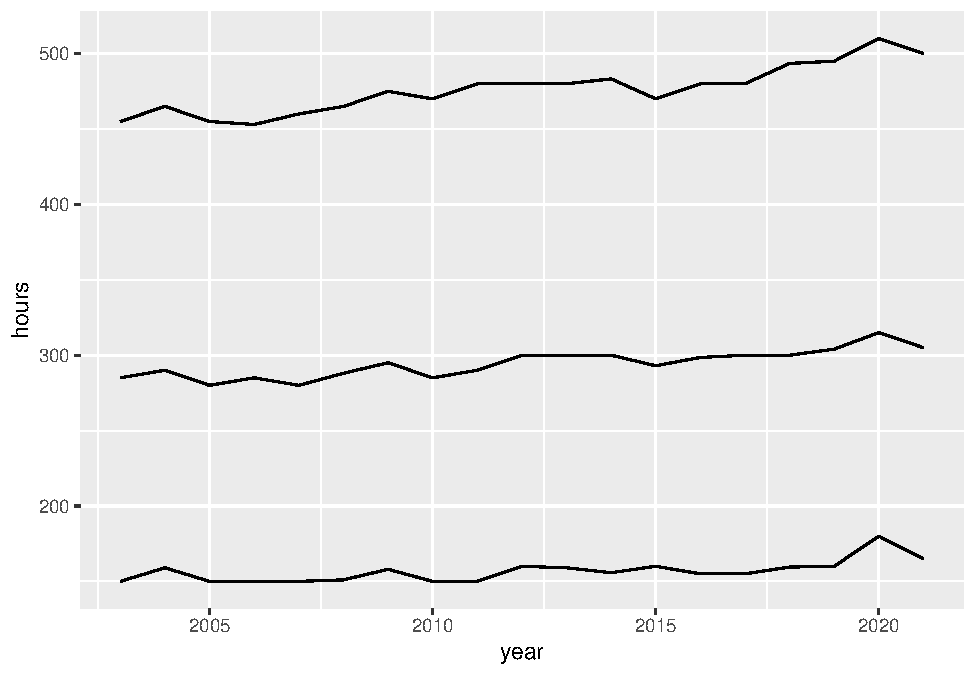
\includegraphics{Paper2_files/figure-latex/graphs-9.pdf}

\begin{Shaded}
\begin{Highlighting}[]
\CommentTok{\# by year, gender}
\NormalTok{csv }\SpecialCharTok{\%\textgreater{}\%}
  \FunctionTok{group\_by}\NormalTok{(year, gender) }\SpecialCharTok{\%\textgreater{}\%}
  \FunctionTok{summarize}\NormalTok{(}\AttributeTok{median =} \FunctionTok{median}\NormalTok{(bls\_leis)) }\SpecialCharTok{\%\textgreater{}\%}
  \FunctionTok{clean\_names}\NormalTok{() }\SpecialCharTok{\%\textgreater{}\%}
  \FunctionTok{filter}\NormalTok{(year }\SpecialCharTok{\textgreater{}} \DecValTok{2005}\NormalTok{) }\SpecialCharTok{\%\textgreater{}\%}
  \FunctionTok{filter}\NormalTok{(year }\SpecialCharTok{\textless{}} \DecValTok{2011}\NormalTok{) }\SpecialCharTok{\%\textgreater{}\%}
  \FunctionTok{ggplot}\NormalTok{(}\FunctionTok{aes}\NormalTok{(}\AttributeTok{x =}\NormalTok{ year, }\AttributeTok{y =}\NormalTok{ median)) }\SpecialCharTok{+}
  \FunctionTok{geom\_line}\NormalTok{() }\SpecialCharTok{+}
  \FunctionTok{facet\_wrap}\NormalTok{(}\SpecialCharTok{\textasciitilde{}}\NormalTok{gender) }\SpecialCharTok{+}
      \FunctionTok{labs}\NormalTok{(}
  \AttributeTok{title =} \StringTok{"Annual individual leisure hours by gender"}\NormalTok{,}
  \AttributeTok{y =} \StringTok{"Annual Hours"}\NormalTok{,}
  \AttributeTok{x =} \StringTok{"Year"}\NormalTok{,}
  \AttributeTok{caption =} \StringTok{"Data from ATUS"}\NormalTok{,}
\NormalTok{) }
\end{Highlighting}
\end{Shaded}

\begin{verbatim}
## `summarise()` has grouped output by 'year'. You can override using the
## `.groups` argument.
\end{verbatim}

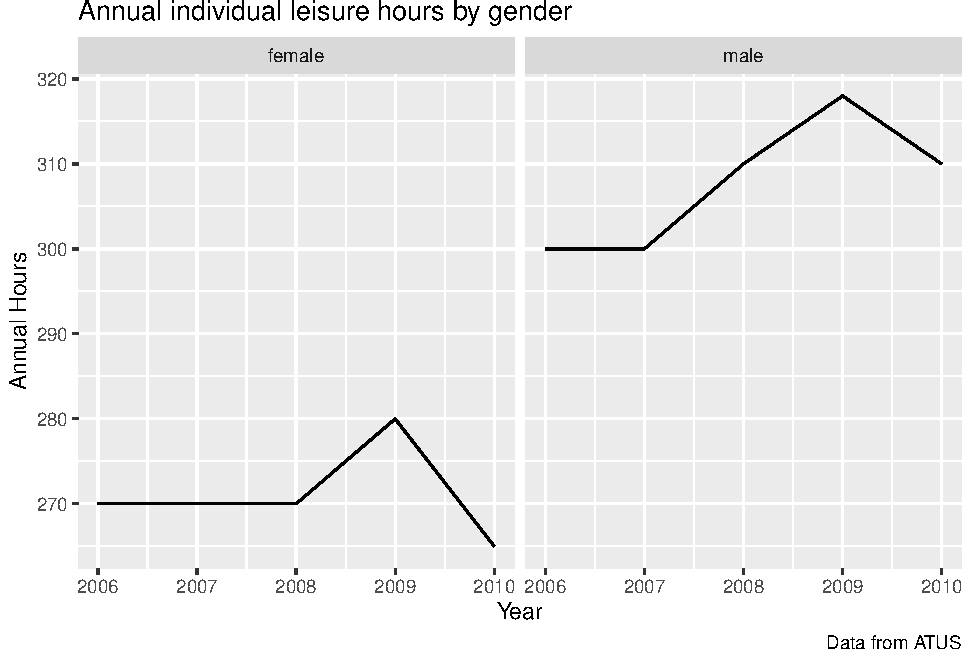
\includegraphics{Paper2_files/figure-latex/graphs-10.pdf}

\begin{Shaded}
\begin{Highlighting}[]
\CommentTok{\#csv \%\textgreater{}\%}
 \CommentTok{\# ggplot(mapping = aes(x = year, y = bls\_leis)) + }
 \CommentTok{\# geom\_jitter(alpha = 0.01)}
\end{Highlighting}
\end{Shaded}

\begin{verbatim}
## # A tibble: 216,683 x 44
##     year  caseid pernum lineno    wt06  wt20   age   sex race_~1 code_~2 code_~3
##    <dbl>   <dbl>  <dbl>  <dbl>   <dbl> <dbl> <dbl> <dbl>   <dbl>   <dbl>   <dbl>
##  1  2003 2.00e13      1      1  8.16e6    NA    60     1     110       1      41
##  2  2003 2.00e13      1      1  1.74e6    NA    41     2     100       1      30
##  3  2003 2.00e13      1      1  3.83e6    NA    26     2     100       2      31
##  4  2003 2.00e13      1      1  6.62e6    NA    36     2     110       1      21
##  5  2003 2.00e13      1      1  3.07e6    NA    51     1     100       1      42
##  6  2003 2.00e13      1      1  3.46e6    NA    32     2     100       4      40
##  7  2003 2.00e13      1      1  1.64e6    NA    44     2     100       3      21
##  8  2003 2.00e13      1      1  6.57e6    NA    21     2     100       6      30
##  9  2003 2.00e13      1      1  1.53e6    NA    33     2     100       1      31
## 10  2003 2.00e13      1      1  4.28e6    NA    39     2     110       1      31
## # ... with 216,673 more rows, 33 more variables: educyrs <dbl>, fullpart <dbl>,
## #   earnweek <dbl>, eldch <dbl>, yngch <dbl>, nchild <dbl>, bls_carehh <dbl>,
## #   bls_comm <dbl>, bls_educ <dbl>, bls_food <dbl>, bls_hhact <dbl>,
## #   bls_leis <dbl>, bls_leis_arts <dbl>, bls_leis_attend <dbl>,
## #   bls_leis_attsport <dbl>, bls_leis_partsport <dbl>, bls_leis_relax <dbl>,
## #   bls_leis_soc <dbl>, bls_leis_soccom <dbl>, bls_leis_soccomex <dbl>,
## #   bls_leis_sport <dbl>, bls_leis_travel <dbl>, bls_leis_tv <dbl>, ...
\end{verbatim}

\begin{verbatim}
## 
## Call:
## lm(formula = bls_leis ~ gender + year + age + race, data = .)
## 
## Coefficients:
##                        (Intercept)                          gendermale  
##                          -623.9103                             49.6546  
##                               year                                 age  
##                             0.3811                              3.6478  
##                     raceAsian only                      raceBlack only  
##                           -63.9278                             22.5268  
##          raceBlack-American Indian  raceHawaiian Pacific Islander only  
##                            -0.8574                            -29.6285  
##                     raceWhite only           raceWhite-American Indian  
##                           -20.1391                             -0.5591  
##                    raceWhite-Asian                     raceWhite-Black  
##                             3.2668                             13.7155  
##                 raceWhite-Hawaiian  
##                           -55.6804
\end{verbatim}

\begin{verbatim}
## 
## Call:
## lm(formula = bls_leis ~ gender + year + age + race, data = .)
## 
## Residuals:
##     Min      1Q  Median      3Q     Max 
## -521.35 -159.52  -31.24  135.26 1135.93 
## 
## Coefficients:
##                                      Estimate Std. Error t value Pr(>|t|)    
## (Intercept)                        -623.91035  167.92625  -3.715 0.000203 ***
## gendermale                           49.65458    0.91800  54.090  < 2e-16 ***
## year                                  0.38115    0.08351   4.564 5.02e-06 ***
## age                                   3.64783    0.02732 133.540  < 2e-16 ***
## raceAsian only                      -63.92776    5.87353 -10.884  < 2e-16 ***
## raceBlack only                       22.52681    5.49110   4.102 4.09e-05 ***
## raceBlack-American Indian            -0.85744   17.09077  -0.050 0.959987    
## raceHawaiian Pacific Islander only  -29.62851   11.37959  -2.604 0.009224 ** 
## raceWhite only                      -20.13907    5.37485  -3.747 0.000179 ***
## raceWhite-American Indian            -0.55913    7.79704  -0.072 0.942833    
## raceWhite-Asian                       3.26685   12.93655   0.253 0.800633    
## raceWhite-Black                      13.71548   11.05354   1.241 0.214673    
## raceWhite-Hawaiian                  -55.68038   26.98951  -2.063 0.039110 *  
## ---
## Signif. codes:  0 '***' 0.001 '**' 0.01 '*' 0.05 '.' 0.1 ' ' 1
## 
## Residual standard error: 211.6 on 216670 degrees of freedom
## Multiple R-squared:  0.09435,    Adjusted R-squared:  0.0943 
## F-statistic:  1881 on 12 and 216670 DF,  p-value: < 2.2e-16
\end{verbatim}

\begin{verbatim}
## # A tibble: 216,683 x 44
##     year  caseid pernum lineno    wt06  wt20   age   sex race_~1 code_~2 code_~3
##    <dbl>   <dbl>  <dbl>  <dbl>   <dbl> <dbl> <dbl> <dbl>   <dbl>   <dbl>   <dbl>
##  1  2003 2.00e13      1      1  8.16e6    NA    60     1     110       1      41
##  2  2003 2.00e13      1      1  1.74e6    NA    41     2     100       1      30
##  3  2003 2.00e13      1      1  3.83e6    NA    26     2     100       2      31
##  4  2003 2.00e13      1      1  6.62e6    NA    36     2     110       1      21
##  5  2003 2.00e13      1      1  3.07e6    NA    51     1     100       1      42
##  6  2003 2.00e13      1      1  3.46e6    NA    32     2     100       4      40
##  7  2003 2.00e13      1      1  1.64e6    NA    44     2     100       3      21
##  8  2003 2.00e13      1      1  6.57e6    NA    21     2     100       6      30
##  9  2003 2.00e13      1      1  1.53e6    NA    33     2     100       1      31
## 10  2003 2.00e13      1      1  4.28e6    NA    39     2     110       1      31
## # ... with 216,673 more rows, 33 more variables: educyrs <dbl>, fullpart <dbl>,
## #   earnweek <dbl>, eldch <dbl>, yngch <dbl>, nchild <dbl>, bls_carehh <dbl>,
## #   bls_comm <dbl>, bls_educ <dbl>, bls_food <dbl>, bls_hhact <dbl>,
## #   bls_leis <dbl>, bls_leis_arts <dbl>, bls_leis_attend <dbl>,
## #   bls_leis_attsport <dbl>, bls_leis_partsport <dbl>, bls_leis_relax <dbl>,
## #   bls_leis_soc <dbl>, bls_leis_soccom <dbl>, bls_leis_soccomex <dbl>,
## #   bls_leis_sport <dbl>, bls_leis_travel <dbl>, bls_leis_tv <dbl>, ...
\end{verbatim}

\begin{verbatim}
## # A tibble: 216,683 x 45
##     year  caseid pernum lineno    wt06  wt20   age   sex race_~1 code_~2 code_~3
##    <dbl>   <dbl>  <dbl>  <dbl>   <dbl> <dbl> <dbl> <dbl>   <dbl>   <dbl>   <dbl>
##  1  2003 2.00e13      1      1  8.16e6    NA    60     1     110       1      41
##  2  2003 2.00e13      1      1  1.74e6    NA    41     2     100       1      30
##  3  2003 2.00e13      1      1  3.83e6    NA    26     2     100       2      31
##  4  2003 2.00e13      1      1  6.62e6    NA    36     2     110       1      21
##  5  2003 2.00e13      1      1  3.07e6    NA    51     1     100       1      42
##  6  2003 2.00e13      1      1  3.46e6    NA    32     2     100       4      40
##  7  2003 2.00e13      1      1  1.64e6    NA    44     2     100       3      21
##  8  2003 2.00e13      1      1  6.57e6    NA    21     2     100       6      30
##  9  2003 2.00e13      1      1  1.53e6    NA    33     2     100       1      31
## 10  2003 2.00e13      1      1  4.28e6    NA    39     2     110       1      31
## # ... with 216,673 more rows, 34 more variables: educyrs <dbl>, fullpart <dbl>,
## #   earnweek <dbl>, eldch <dbl>, yngch <dbl>, nchild <dbl>, bls_carehh <dbl>,
## #   bls_comm <dbl>, bls_educ <dbl>, bls_food <dbl>, bls_hhact <dbl>,
## #   bls_leis <dbl>, bls_leis_arts <dbl>, bls_leis_attend <dbl>,
## #   bls_leis_attsport <dbl>, bls_leis_partsport <dbl>, bls_leis_relax <dbl>,
## #   bls_leis_soc <dbl>, bls_leis_soccom <dbl>, bls_leis_soccomex <dbl>,
## #   bls_leis_sport <dbl>, bls_leis_travel <dbl>, bls_leis_tv <dbl>, ...
\end{verbatim}

\begin{verbatim}
## 
## Call:
## lm(formula = bls_leis ~ gender + year + age + race + new_educ, 
##     data = .)
## 
## Residuals:
##     Min      1Q  Median      3Q     Max 
## -540.08 -157.16  -30.31  134.72 1125.90 
## 
## Coefficients:
##                                      Estimate Std. Error t value Pr(>|t|)    
## (Intercept)                        -1.465e+03  1.675e+02  -8.743  < 2e-16 ***
## gendermale                          5.018e+01  9.120e-01  55.024  < 2e-16 ***
## year                                8.183e-01  8.335e-02   9.818  < 2e-16 ***
## age                                 3.516e+00  2.727e-02 128.908  < 2e-16 ***
## raceAsian only                     -3.776e+01  5.855e+00  -6.449 1.13e-10 ***
## raceBlack only                      2.835e+01  5.455e+00   5.197 2.03e-07 ***
## raceBlack-American Indian           5.276e+00  1.698e+01   0.311   0.7560    
## raceHawaiian Pacific Islander only -1.861e+01  1.130e+01  -1.646   0.0997 .  
## raceWhite only                     -7.804e+00  5.344e+00  -1.460   0.1442    
## raceWhite-American Indian           5.349e+00  7.746e+00   0.691   0.4898    
## raceWhite-Asian                     2.130e+01  1.285e+01   1.657   0.0975 .  
## raceWhite-Black                     2.235e+01  1.098e+01   2.035   0.0418 *  
## raceWhite-Hawaiian                 -4.264e+01  2.681e+01  -1.590   0.1117    
## new_educ>Four Year Degree          -7.571e+01  1.611e+00 -46.994  < 2e-16 ***
## new_educHigh School Graduate       -3.253e+01  1.524e+00 -21.351  < 2e-16 ***
## ---
## Signif. codes:  0 '***' 0.001 '**' 0.01 '*' 0.05 '.' 0.1 ' ' 1
## 
## Residual standard error: 210.2 on 216668 degrees of freedom
## Multiple R-squared:  0.1065, Adjusted R-squared:  0.1064 
## F-statistic:  1844 on 14 and 216668 DF,  p-value: < 2.2e-16
\end{verbatim}

\begin{verbatim}
## # A tibble: 216,683 x 45
##     year  caseid pernum lineno    wt06  wt20   age   sex race_~1 code_~2 code_~3
##    <dbl>   <dbl>  <dbl>  <dbl>   <dbl> <dbl> <dbl> <dbl>   <dbl>   <dbl>   <dbl>
##  1  2003 2.00e13      1      1  8.16e6    NA    60     1     110       1      41
##  2  2003 2.00e13      1      1  1.74e6    NA    41     2     100       1      30
##  3  2003 2.00e13      1      1  3.83e6    NA    26     2     100       2      31
##  4  2003 2.00e13      1      1  6.62e6    NA    36     2     110       1      21
##  5  2003 2.00e13      1      1  3.07e6    NA    51     1     100       1      42
##  6  2003 2.00e13      1      1  3.46e6    NA    32     2     100       4      40
##  7  2003 2.00e13      1      1  1.64e6    NA    44     2     100       3      21
##  8  2003 2.00e13      1      1  6.57e6    NA    21     2     100       6      30
##  9  2003 2.00e13      1      1  1.53e6    NA    33     2     100       1      31
## 10  2003 2.00e13      1      1  4.28e6    NA    39     2     110       1      31
## # ... with 216,673 more rows, 34 more variables: educyrs <dbl>, fullpart <dbl>,
## #   earnweek <dbl>, eldch <dbl>, yngch <dbl>, nchild <dbl>, bls_carehh <dbl>,
## #   bls_comm <dbl>, bls_educ <dbl>, bls_food <dbl>, bls_hhact <dbl>,
## #   bls_leis <dbl>, bls_leis_arts <dbl>, bls_leis_attend <dbl>,
## #   bls_leis_attsport <dbl>, bls_leis_partsport <dbl>, bls_leis_relax <dbl>,
## #   bls_leis_soc <dbl>, bls_leis_soccom <dbl>, bls_leis_soccomex <dbl>,
## #   bls_leis_sport <dbl>, bls_leis_travel <dbl>, bls_leis_tv <dbl>, ...
\end{verbatim}

\begin{verbatim}
## 
## Call:
## lm(formula = bls_leis ~ gender + year + age + race + new_educ + 
##     nchild, data = .)
## 
## Residuals:
##     Min      1Q  Median      3Q     Max 
## -539.73 -154.35  -29.01  133.50 1119.92 
## 
## Coefficients:
##                                      Estimate Std. Error t value Pr(>|t|)    
## (Intercept)                        -1.166e+03  1.660e+02  -7.027 2.12e-12 ***
## gendermale                          4.745e+01  9.041e-01  52.479  < 2e-16 ***
## year                                7.034e-01  8.256e-02   8.520  < 2e-16 ***
## age                                 2.801e+00  2.914e-02  96.120  < 2e-16 ***
## raceAsian only                     -3.911e+01  5.798e+00  -6.746 1.52e-11 ***
## raceBlack only                      2.046e+01  5.404e+00   3.786 0.000153 ***
## raceBlack-American Indian           1.239e+00  1.681e+01   0.074 0.941243    
## raceHawaiian Pacific Islander only -1.644e+01  1.120e+01  -1.469 0.141879    
## raceWhite only                     -1.060e+01  5.292e+00  -2.003 0.045178 *  
## raceWhite-American Indian           1.489e-01  7.671e+00   0.019 0.984508    
## raceWhite-Asian                     1.063e+01  1.273e+01   0.835 0.403774    
## raceWhite-Black                     1.742e+01  1.087e+01   1.602 0.109231    
## raceWhite-Hawaiian                 -3.995e+01  2.655e+01  -1.505 0.132373    
## new_educ>Four Year Degree          -7.832e+01  1.596e+00 -49.076  < 2e-16 ***
## new_educHigh School Graduate       -3.773e+01  1.511e+00 -24.971  < 2e-16 ***
## nchild                             -2.819e+01  4.313e-01 -65.352  < 2e-16 ***
## ---
## Signif. codes:  0 '***' 0.001 '**' 0.01 '*' 0.05 '.' 0.1 ' ' 1
## 
## Residual standard error: 208.2 on 216667 degrees of freedom
## Multiple R-squared:  0.1238, Adjusted R-squared:  0.1237 
## F-statistic:  2040 on 15 and 216667 DF,  p-value: < 2.2e-16
\end{verbatim}

\begin{verbatim}
## 
## Call:
## lm(formula = bls_leis ~ gender + year + age + race + new_educ + 
##     nchild + marst_simple, data = .)
## 
## Residuals:
##     Min      1Q  Median      3Q     Max 
## -559.24 -153.58  -28.34  133.35 1112.47 
## 
## Coefficients:
##                                      Estimate Std. Error t value Pr(>|t|)    
## (Intercept)                        -827.70534  165.76859  -4.993 5.95e-07 ***
## gendermale                           49.21292    0.90980  54.092  < 2e-16 ***
## year                                  0.51202    0.08251   6.206 5.46e-10 ***
## age                                   3.16552    0.03357  94.297  < 2e-16 ***
## raceAsian only                      -32.06597    5.78459  -5.543 2.97e-08 ***
## raceBlack only                       16.45575    5.38889   3.054  0.00226 ** 
## raceBlack-American Indian            -2.10998   16.76170  -0.126  0.89983    
## raceHawaiian Pacific Islander only  -14.46619   11.16218  -1.296  0.19498    
## raceWhite only                       -6.52367    5.27747  -1.236  0.21641    
## raceWhite-American Indian             2.39777    7.64806   0.314  0.75389    
## raceWhite-Asian                      12.24182   12.69238   0.965  0.33480    
## raceWhite-Black                      15.28628   10.84182   1.410  0.15856    
## raceWhite-Hawaiian                  -39.51993   26.46932  -1.493  0.13543    
## new_educ>Four Year Degree           -72.84907    1.60042 -45.519  < 2e-16 ***
## new_educHigh School Graduate        -34.95019    1.50857 -23.168  < 2e-16 ***
## nchild                              -21.28270    0.47146 -45.142  < 2e-16 ***
## marst_simpleNever Married            46.52934    1.35044  34.455  < 2e-16 ***
## marst_simpleSeparated/Divorced       22.65070    1.14949  19.705  < 2e-16 ***
## ---
## Signif. codes:  0 '***' 0.001 '**' 0.01 '*' 0.05 '.' 0.1 ' ' 1
## 
## Residual standard error: 207.5 on 216665 degrees of freedom
## Multiple R-squared:  0.129,  Adjusted R-squared:  0.1289 
## F-statistic:  1888 on 17 and 216665 DF,  p-value: < 2.2e-16
\end{verbatim}

\begin{verbatim}
## 
## % Table created by stargazer v.5.2.3 by Marek Hlavac, Social Policy Institute. E-mail: marek.hlavac at gmail.com
## % Date and time: Mon, Nov 28, 2022 - 01:29:04
## % Requires LaTeX packages: dcolumn 
## \begin{table}[!htbp] \centering 
##   \caption{Various Models} 
##   \label{} 
## \begin{tabular}{@{\extracolsep{5pt}}lD{.}{.}{-3} D{.}{.}{-3} D{.}{.}{-3} } 
## \\[-1.8ex]\hline 
## \hline \\[-1.8ex] 
##  & \multicolumn{3}{c}{\textit{Dependent variable:}} \\ 
## \cline{2-4} 
## \\[-1.8ex] & \multicolumn{3}{c}{bls\_leis} \\ 
## \\[-1.8ex] & \multicolumn{1}{c}{(1)} & \multicolumn{1}{c}{(2)} & \multicolumn{1}{c}{(3)}\\ 
## \hline \\[-1.8ex] 
##  gendermale & 44.200^{***} & 43.935^{***} & 49.655^{***} \\ 
##   & (0.958) & (0.957) & (0.918) \\ 
##   & & & \\ 
##  year &  & 1.458^{***} & 0.381^{***} \\ 
##   &  & (0.087) & (0.084) \\ 
##   & & & \\ 
##  age &  &  & 3.648^{***} \\ 
##   &  &  & (0.027) \\ 
##   & & & \\ 
##  raceAsian only &  &  & -63.928^{***} \\ 
##   &  &  & (5.874) \\ 
##   & & & \\ 
##  raceBlack only &  &  & 22.527^{***} \\ 
##   &  &  & (5.491) \\ 
##   & & & \\ 
##  raceBlack-American Indian &  &  & -0.857 \\ 
##   &  &  & (17.091) \\ 
##   & & & \\ 
##  raceHawaiian Pacific Islander only &  &  & -29.629^{***} \\ 
##   &  &  & (11.380) \\ 
##   & & & \\ 
##  raceWhite only &  &  & -20.139^{***} \\ 
##   &  &  & (5.375) \\ 
##   & & & \\ 
##  raceWhite-American Indian &  &  & -0.559 \\ 
##   &  &  & (7.797) \\ 
##   & & & \\ 
##  raceWhite-Asian &  &  & 3.267 \\ 
##   &  &  & (12.937) \\ 
##   & & & \\ 
##  raceWhite-Black &  &  & 13.715 \\ 
##   &  &  & (11.054) \\ 
##   & & & \\ 
##  raceWhite-Hawaiian &  &  & -55.680^{**} \\ 
##   &  &  & (26.990) \\ 
##   & & & \\ 
##  Constant & 310.025^{***} & -2,621.242^{***} & -623.910^{***} \\ 
##   & (0.634) & (174.290) & (167.926) \\ 
##   & & & \\ 
## \hline \\[-1.8ex] 
## Observations & \multicolumn{1}{c}{216,908} & \multicolumn{1}{c}{216,908} & \multicolumn{1}{c}{216,683} \\ 
## R$^{2}$ & \multicolumn{1}{c}{0.010} & \multicolumn{1}{c}{0.011} & \multicolumn{1}{c}{0.094} \\ 
## Adjusted R$^{2}$ & \multicolumn{1}{c}{0.010} & \multicolumn{1}{c}{0.011} & \multicolumn{1}{c}{0.094} \\ 
## Residual Std. Error & \multicolumn{1}{c}{221.309 (df = 216906)} & \multicolumn{1}{c}{221.166 (df = 216905)} & \multicolumn{1}{c}{211.630 (df = 216670)} \\ 
## F Statistic & \multicolumn{1}{c}{2,129.097$^{***}$ (df = 1; 216906)} & \multicolumn{1}{c}{1,207.362$^{***}$ (df = 2; 216905)} & \multicolumn{1}{c}{1,880.976$^{***}$ (df = 12; 216670)} \\ 
## \hline 
## \hline \\[-1.8ex] 
## \textit{Note:}  & \multicolumn{3}{r}{$^{*}$p$<$0.1; $^{**}$p$<$0.05; $^{***}$p$<$0.01} \\ 
## \end{tabular} 
## \end{table}
\end{verbatim}

\begin{Shaded}
\begin{Highlighting}[]
\CommentTok{\#Change}

\NormalTok{change }\OtherTok{\textless{}{-}}\NormalTok{ newcsv1 }\SpecialCharTok{\%\textgreater{}\%}
  \FunctionTok{group\_by}\NormalTok{(gender,  year, new\_educ, child, marst\_simple) }\SpecialCharTok{\%\textgreater{}\%}
  \FunctionTok{summarize}\NormalTok{(}\FunctionTok{median}\NormalTok{(bls\_leis)) }\SpecialCharTok{\%\textgreater{}\%}
  \FunctionTok{clean\_names}\NormalTok{() }\SpecialCharTok{\%\textgreater{}\%}
  \FunctionTok{pivot\_wider}\NormalTok{(}\AttributeTok{values\_from =}\NormalTok{ median\_bls\_leis, }\AttributeTok{names\_from =}\NormalTok{ year) }\SpecialCharTok{\%\textgreater{}\%}
  \FunctionTok{clean\_names}\NormalTok{() }\SpecialCharTok{\%\textgreater{}\%}
  \FunctionTok{mutate}\NormalTok{(}\AttributeTok{leisure\_change =}\NormalTok{ x2009 }\SpecialCharTok{{-}}\NormalTok{ x2007)}
\end{Highlighting}
\end{Shaded}

\begin{verbatim}
## `summarise()` has grouped output by 'gender', 'year', 'new_educ', 'child'. You
## can override using the `.groups` argument.
\end{verbatim}

\begin{Shaded}
\begin{Highlighting}[]
\NormalTok{change2 }\OtherTok{\textless{}{-}}\NormalTok{ newcsv1 }\SpecialCharTok{\%\textgreater{}\%}
  \FunctionTok{group\_by}\NormalTok{(gender, year) }\SpecialCharTok{\%\textgreater{}\%}
  \FunctionTok{summarize}\NormalTok{(}\FunctionTok{median}\NormalTok{(bls\_leis)) }\SpecialCharTok{\%\textgreater{}\%}
  \FunctionTok{clean\_names}\NormalTok{() }\SpecialCharTok{\%\textgreater{}\%}
  \FunctionTok{pivot\_wider}\NormalTok{(}\AttributeTok{values\_from =}\NormalTok{ median\_bls\_leis, }\AttributeTok{names\_from =}\NormalTok{ year) }\SpecialCharTok{\%\textgreater{}\%}
  \FunctionTok{clean\_names}\NormalTok{() }\SpecialCharTok{\%\textgreater{}\%}
  \FunctionTok{mutate}\NormalTok{(}\AttributeTok{leisure\_change =}\NormalTok{ x2009 }\SpecialCharTok{{-}}\NormalTok{ x2007)}
\end{Highlighting}
\end{Shaded}

\begin{verbatim}
## `summarise()` has grouped output by 'gender'. You can override using the
## `.groups` argument.
\end{verbatim}

\begin{Shaded}
\begin{Highlighting}[]
\NormalTok{change2}
\end{Highlighting}
\end{Shaded}

\begin{verbatim}
## # A tibble: 2 x 21
## # Groups:   gender [2]
##   gender x2003 x2004 x2005 x2006 x2007 x2008 x2009 x2010 x2011 x2012 x2013 x2014
##   <chr>  <dbl> <dbl> <dbl> <dbl> <dbl> <dbl> <dbl> <dbl> <dbl> <dbl> <dbl> <dbl>
## 1 female   270   270   270   270   270   270   280   266   275   285   280   280
## 2 male     300   315   300   300   300   310   318   310   303   330   320   320
## # ... with 8 more variables: x2015 <dbl>, x2016 <dbl>, x2017 <dbl>,
## #   x2018 <dbl>, x2019 <dbl>, x2020 <dbl>, x2021 <dbl>, leisure_change <dbl>
\end{verbatim}

\begin{Shaded}
\begin{Highlighting}[]
\NormalTok{delta }\OtherTok{\textless{}{-}}\NormalTok{ change }\SpecialCharTok{\%\textgreater{}\%}
  \FunctionTok{lm}\NormalTok{(}\AttributeTok{formula =}\NormalTok{ leisure\_change }\SpecialCharTok{\textasciitilde{}}\NormalTok{ gender}\SpecialCharTok{+}\NormalTok{ new\_educ}\SpecialCharTok{+}\NormalTok{ child}\SpecialCharTok{+}\NormalTok{ marst\_simple)}
\FunctionTok{summary}\NormalTok{(delta)}
\end{Highlighting}
\end{Shaded}

\begin{verbatim}
## 
## Call:
## lm(formula = leisure_change ~ gender + new_educ + child + marst_simple, 
##     data = .)
## 
## Residuals:
##     Min      1Q  Median      3Q     Max 
## -79.708 -30.594  -0.549  18.368 148.556 
## 
## Coefficients:
##                                Estimate Std. Error t value Pr(>|t|)  
## (Intercept)                      28.569     22.031   1.297   0.2049  
## gendermale                       13.194     16.654   0.792   0.4346  
## new_educ>Four Year Degree       -38.542     20.397  -1.890   0.0689 .
## new_educHigh School Graduate    -45.417     20.397  -2.227   0.0339 *
## child                             7.639     16.654   0.459   0.6499  
## marst_simpleNever Married        14.750     20.397   0.723   0.4754  
## marst_simpleSeparated/Divorced   33.542     20.397   1.644   0.1109  
## ---
## Signif. codes:  0 '***' 0.001 '**' 0.01 '*' 0.05 '.' 0.1 ' ' 1
## 
## Residual standard error: 49.96 on 29 degrees of freedom
## Multiple R-squared:  0.2431, Adjusted R-squared:  0.08656 
## F-statistic: 1.553 on 6 and 29 DF,  p-value: 0.1966
\end{verbatim}

\end{document}
